\documentclass[unicode, notheorems]{beamer}
\usepackage{etex}  % Should be second line. Otherwise tikz raises error.
\hypersetup{pdfpagemode=FullScreen}

% If you have more than three sections or more than three subsections in at least one section,
% you might want to use the [compress] switch. In this case, only the current (sub-) section
% is displayed in the header and not the full overview.
\mode<presentation>
{
  \usetheme{Madrid}
  \usecolortheme{seahorse}
}

% https://tex.stackexchange.com/questions/106789/why-does-usepackaget2afontenc-take-over
\usepackage[T2A,T1]{fontenc}
\usepackage[english]{babel}
\usepackage{amsthm}
\usepackage[noend]{algorithmic}
\usepackage{algorithm}
\usepackage[all]{xy} % for graph plotting
% \usepackage{times}
\usepackage{tikz}
\usetikzlibrary{arrows,shapes,backgrounds}
\usepackage{textcomp} % euro sign
\usepackage[official]{eurosym}
\usepackage{ulem} % strike
\usepackage{color} % use colors (in minted)

% tables
\usepackage{booktabs}
\usepackage{multirow}

%% Code highlight
% Doc: http://ftp.yzu.edu.tw/CTAN/macros/latex/contrib/listings/listings.pdf
\usepackage{listings}
\usepackage{minted}
\definecolor{LightGray}{rgb}{0.9,0.9,0.9}
%\setminted{bgcolor=LightGray}
%\usemintedstyle{monokai}
% ftp://ftp.dante.de/tex-archive/macros/latex/contrib/minted/minted.pdf
% Note: to use minted, install pygments http://pygments.org/ and add "-shell-escape" flag to latex command.
% Minted doc: http://ftp.yzu.edu.tw/CTAN/macros/latex/contrib/minted/minted.pdf
%% END: Code highlight

% Font settings 
%\usepackage[scaled]{futura}
\usepackage{helvet}

%\usefonttheme{serif}     % Font theme: serif
%\usepackage{ccfonts}     % Font family: Concrete Math

% \usefonttheme[onlymath]{serif}
% \defaultfontfeatures{Mapping=tex-text} 
%\setsansfont[Ligatures={Common}]{Futura}
% \setmonofont[Scale=0.8]{Monaco} 

\title{Apache Spark in Data Science}
\subtitle{Real World Applications}
\author{Kirill Pavlov}
\institute[]{Data Science Team, Asia Miles Limited}
\titlegraphic{
\includegraphics[width=4cm]{./images/logo}}
\date{May 12, 2016}

\definecolor{aml_gray_light}{RGB}{147,153,157}
\definecolor{aml_gray_dark}{RGB}{39,47,56}
\definecolor{aml_yellow}{RGB}{250,207,0}

\setbeamertemplate{title page}[default][colsep=-4bp,rounded=true]
\setbeamertemplate{itemize items}[default]
\setbeamertemplate{enumerate items}[default]

\setbeamercolor*{palette primary}{use=structure,fg=white,bg=aml_gray_light}
\setbeamercolor*{palette secondary}{use=structure,fg=white,bg=aml_gray_dark}
\setbeamercolor*{palette tertiary}{use=structure,fg=white,bg=aml_yellow}

\setbeamercolor{itemize item}{fg=aml_yellow}
\setbeamercolor{itemize subitem}{fg=aml_yellow}
\setbeamercolor{enumerate item}{fg=aml_gray_dark}
\setbeamercolor{enumerate subitem}{fg=aml_gray_dark}

\setbeamertemplate{section in toc}{%
  {\color{aml_gray_dark}\inserttocsectionnumber.}~\inserttocsection}
\setbeamercolor{subsection in toc}{bg=white,fg=structure}
\setbeamertemplate{subsection in toc}{%
  \hspace{1.2em}{\color{aml_gray_dark}\rule[0.3ex]{3pt}{3pt}}~\inserttocsubsection\par}
  
% Set beamer blocks
\setbeamertemplate{blocks}[rounded][shadow=false]
\addtobeamertemplate{block begin}{\pgfsetfillopacity{0.8}}{\pgfsetfillopacity{1}}

% \setbeamercolor*{block title example}{fg=aml_gray_dark,bg= aml_gray_light}
%\setbeamercolor*{block body example}{fg= blue,bg= blue!5}
\setbeamercolor*{block title example}{fg=white,bg= aml_gray_light}
\setbeamercolor*{block body example}{fg=white,bg= aml_gray_dark}

% remove page navigation.
\beamertemplatenavigationsymbolsempty

% Set link colours
\definecolor{links}{HTML}{2A1B81}
\hypersetup{colorlinks,linkcolor=,urlcolor=links}

\begin{document}
% For every picture that defines or uses external nodes, you'll have to
% apply the 'remember picture' style. To avoid some typing, we'll apply
% the style to all pictures.
\tikzstyle{every picture}+=[remember picture]

% By default all math in TikZ nodes are set in inline mode. Change this to
% displaystyle so that we don't get small fractions.
\everymath{\displaystyle}

% This presentation shows ability of spark to work with data.
% It covers data processing, pipelining, feature engineering and algorithms available in Spark.

\begin{frame}
\titlepage
\end{frame}


\begin{frame}{Disclaimer}
The opinions expressed in this presentation and on the following slides are solely those of the presenter and not necessarily those of Asia Miles Limited.
\end{frame}


\begin{frame}{Quick Questionnaire}
\begin{itemize}
\item How many people have attended previous Spark talks? \pause
\item How many people are currently working with Spark? \pause
\item How many people are familiar with Scala?
\end{itemize}
\end{frame}


\begin{frame}{About the Presenter}
\begin{columns}
\column{.7\textwidth}
  {\footnotesize 
    \begin{itemize}
    \item MS degree from Moscow Institute of Physics and Technology with distinction.
    \item 8+ years of data science and machine learning experience.
    \item Worked in Yandex (Russian Google) on search and on-line contextual ads ranking algorithms.
    \item Developed and consulted start-ups in digital marketing, healthcare, real estate and home automation areas.
    \item Open-source contributor, full-stack engineer and data mining evangelist.
    \item Now data scientist in Asia Miles.
    \end{itemize}
  }
\column{.3\textwidth}
	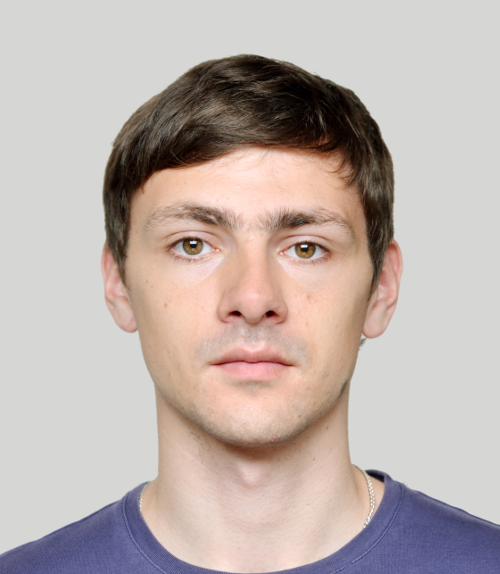
\includegraphics[scale=0.8]{images/author}
\end{columns}
\end{frame}


{
\usebackgroundtemplate{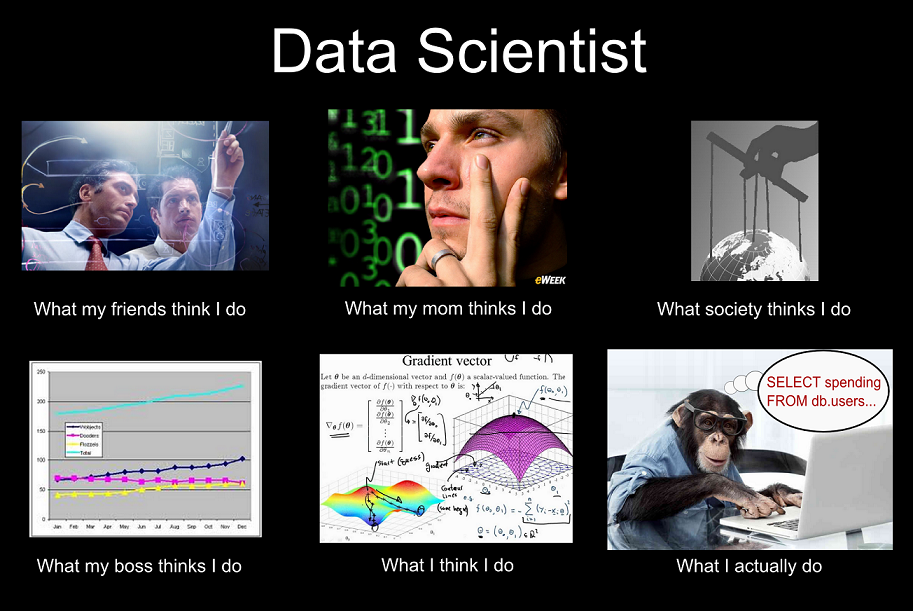
\includegraphics[width=\paperwidth,height=\paperheight]{./images/Data-Scientist-What-I-really-do}}
\begin{frame}[plain]
%% Some of you may know about this picture. I would like to focus on its bottom part. My boss thinks I am working with excel. Thank is not necesserely wrong. Problem with "what I do" picture is that people do not understand it. After part with formulas we simple charts.
%% Another picture I would like to focus here is "what I actually do", particulary SQL part, which is seems to be nesessary for big data projects.

%\vfill
%{\footnotesize
%\color[rgb]{1,1,1}{source:} \href{http://www.sintetia.com/wp-content/uploads/2014/05/Data-Scientist-What-I-really-do.png}{\color[rgb]{1,1,1}{www.sintetia.com}}
%}
\end{frame}
}


\begin{frame}{Data Scientist skills}
\begin{columns}
\column{.33\textwidth}
\begin{center}
	
\includegraphics[height=3.5cm]{images/software-developer}
\end{center}
\begin{center}
Software Engineering
\end{center}
\column{.33\textwidth}
\begin{center}
	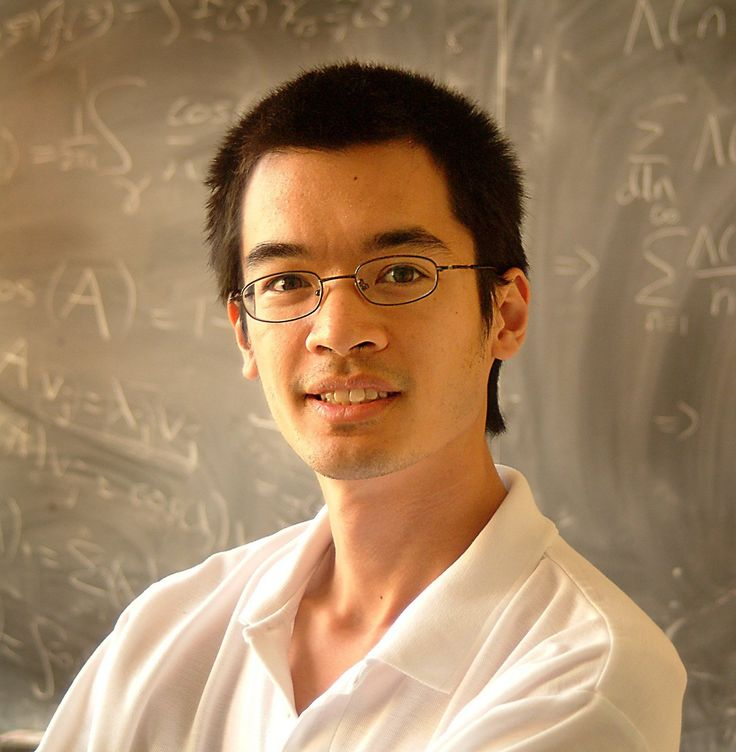
\includegraphics[height=3.5cm]{images/scientist}
\end{center}
\begin{center}
Data Mining
\end{center}
\column{.34\textwidth}
\begin{center}
	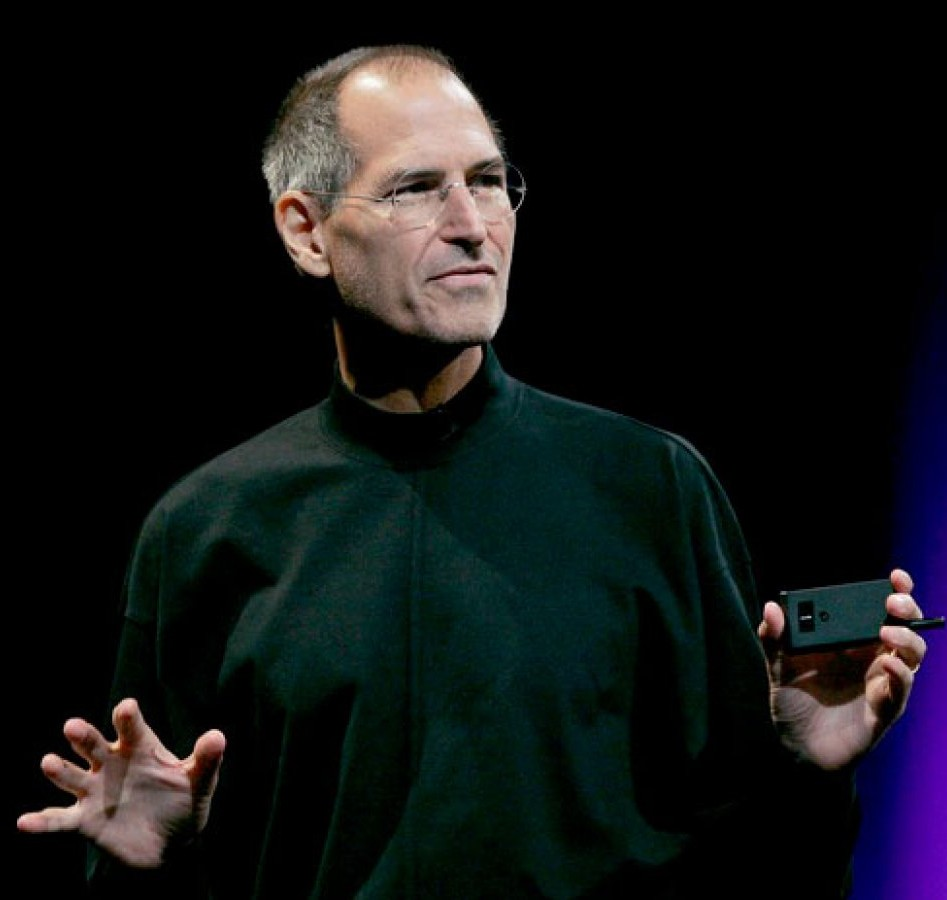
\includegraphics[height=3.5cm]{images/presenter}
\end{center}
\begin{center}
Presentation
\end{center}
\end{columns}
\end{frame}


\begin{frame}{Table of content}
  % \tableofcontents[currentsection]
  \tableofcontents
\end{frame}


\section{Overview}
\begin{frame}{Table of content}
\tableofcontents[currentsection]
\end{frame}
%\frame{\tableofcontents[currentsection]}


\begin{frame}{Environment}
\begin{columns}
\column{.33\textwidth}
\begin{center}
	
\includegraphics[scale=0.5]{images/spark}
\end{center}
\column{.33\textwidth}
\begin{center}
	
\includegraphics[scale=0.5]{images/scala}
\end{center}
\column{.34\textwidth}
\begin{center}
	
\includegraphics[scale=0.5]{images/zeppelin}
\end{center}
\end{columns}

% * How do we work with spark in the private cloud: zeppelin. Why zeppelin?
% * We use scala. Why not python? native integration.
% * Why zeppelin? (notebook at all/compare to Jupyter)
\end{frame}


\begin{frame}{Spark connection with other tools}
\begin{center}
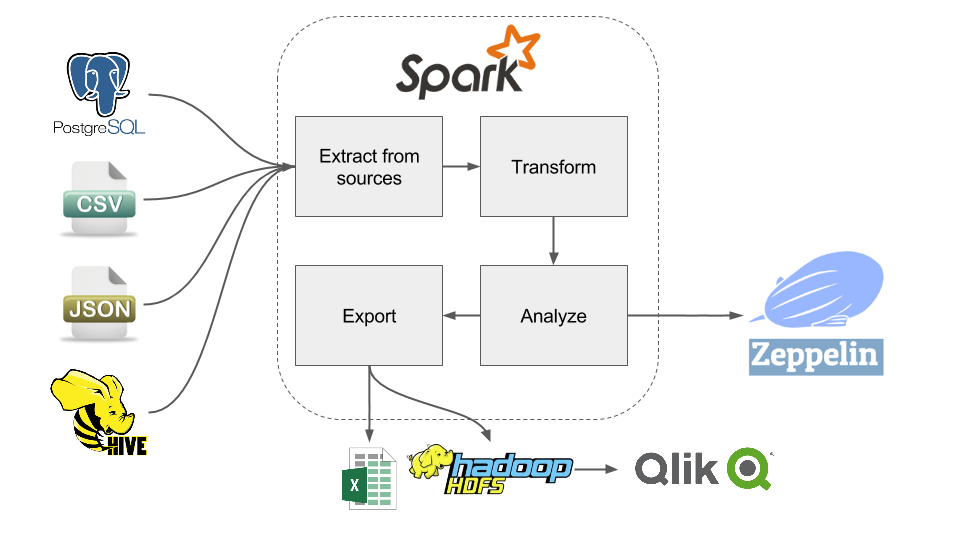
\includegraphics[width=12.5cm]{images/spark-overview}
\end{center}
\end{frame}


%\subsection{Engineering}
\begin{frame}{Software Engineering}

\begin{columns}
\column{.25\textwidth}
\begin{center}
	
\includegraphics[width=3.2cm]{images/software-developer}
\end{center}
\column{.75\textwidth}

\begin{itemize}
\item External libraries could be included to spark-submit and Zeppelin from \href{http://mvnrepository.com/}{mvn repository}. \pause
\item Internal libraries are continuously tested and packaged to JARs. \pause
\item Frequent tasks are executed with schedulers, such as \href{https://pythonhosted.org/airflow/}{Airflow}.
\end{itemize}
\end{columns}
\end{frame}


\begin{frame}[fragile]{External JARs usage}
Example of spark-submit with dependencies:

\begin{minted}[bgcolor=LightGray]{shell}
spark-submit --master yarn \
  --jars spark-csv_2.11.jar,dependency.jar \
  --class com.example.ComputeSomething \
  mypackage.jar
\end{minted}

\vfill
Zeppelin example:

\begin{minted}[escapeinside=||,bgcolor=LightGray]{scala}
|\%|dep
z.load("/path/to/spark-csv_2.11.jar")
z.load("/path/to/dependency.jar")
\end{minted}
\end{frame}


%\subsection{Data visualization}
\begin{frame}{Visualization}
\begin{columns}
\column{.25\textwidth}
\begin{center}
	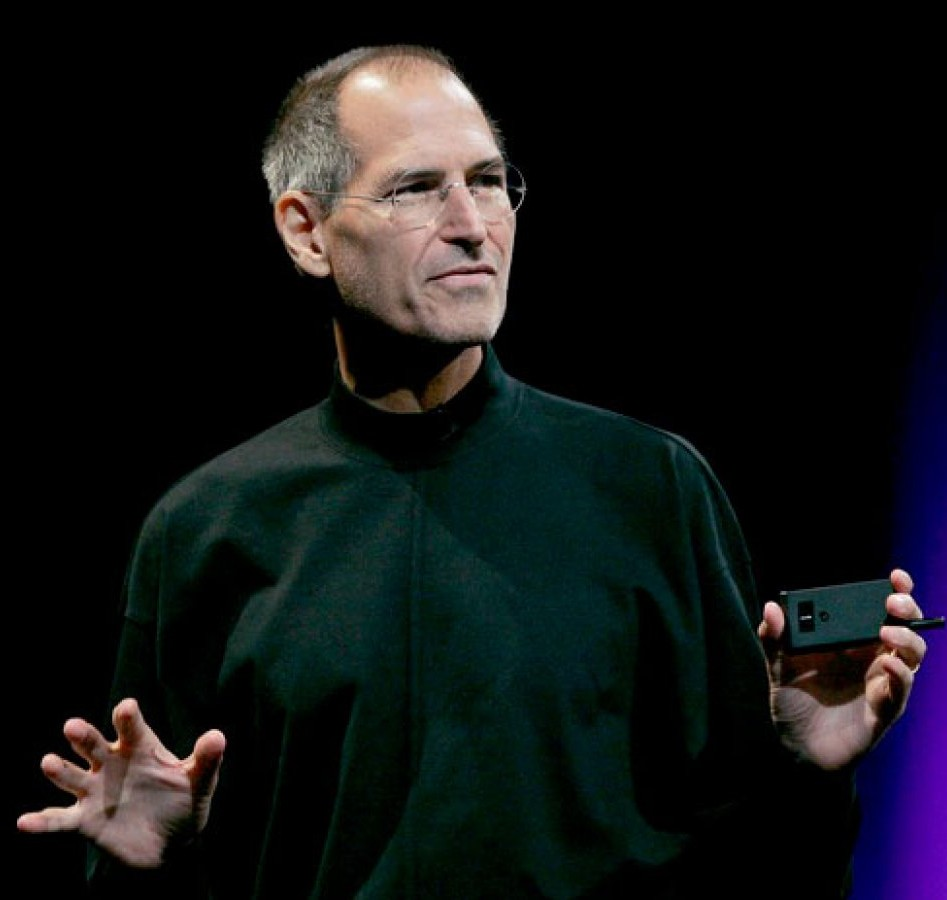
\includegraphics[width=3.2cm]{images/presenter}
\end{center}
\column{.75\textwidth}

\begin{itemize}
\item Data generation and visualization are two \textbf{independent} components. \pause % different tools for each of them
\item Neither of Spark/Python/R produces easy customizable charts. \pause %They are used for exploratory, but not for explanatory analysis.
\item Solution: BI dashboards (QlikView, Tableau) and Excel. Sometimes JavaScript (d3js, MapBox) works better.
\end{itemize}

\end{columns}
% Data visualization split data generation from data plot. Automate genration part.
% BI tools (write data back to DB or export to csv, etc.)
\end{frame}


\begin{frame}{Visualization}
\begin{center}
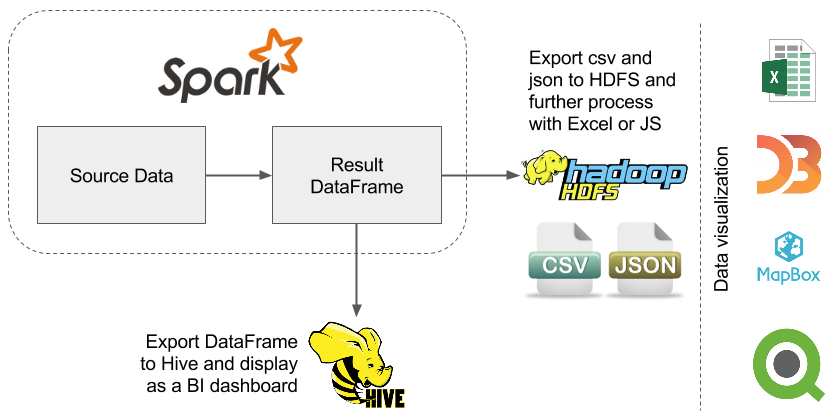
\includegraphics[width=12cm]{images/visualization}
\end{center}
\end{frame}


\section{Data transformation with Spark}
\begin{frame}{Table of content}
\tableofcontents[currentsection]
\end{frame}
\begin{frame}{Data manipulation options}
\begin{itemize}
\item Spark.
\item MapReduce/Hive.
\item RDBMS: Postgres/MySQL/etc.
\item Pandas/R DataFrames.
\end{itemize}
\end{frame}

\begin{frame}{Persistent storage options}
\begin{itemize}
\item Hive: out of the box fast access to the data.
\item HDFS ORC: data could be partitioned.
\item HDFS CSV: easy to export to local file system.
\end{itemize}
\begin{center}
	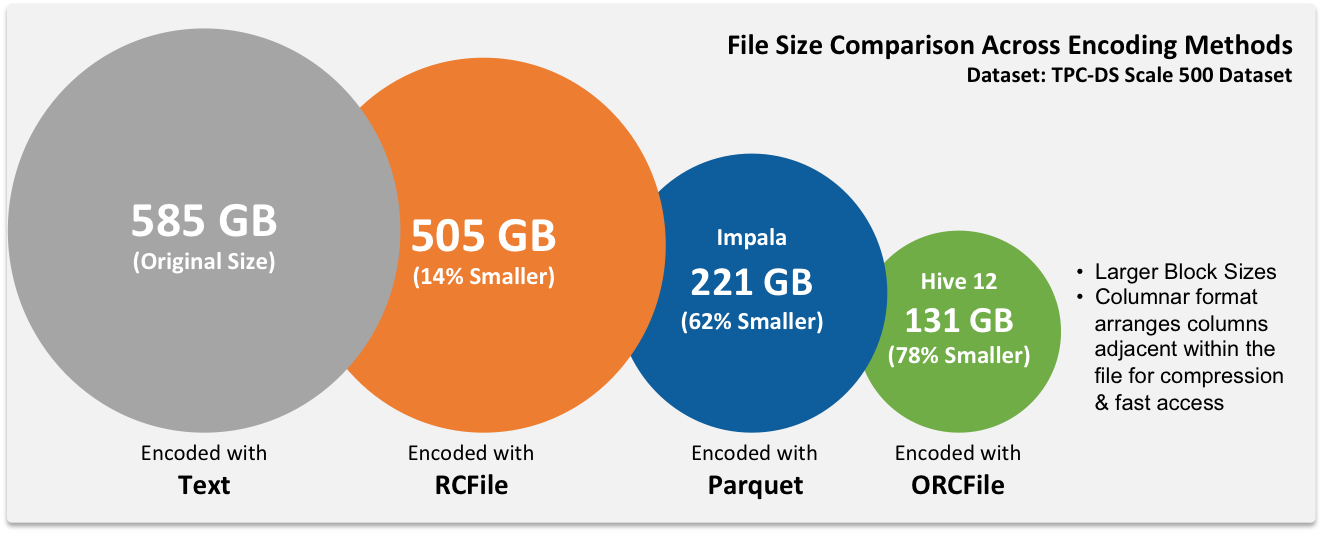
\includegraphics[width=10cm, height=4cm]{images/storage-formats}
\end{center}
\end{frame}

%\begin{frame}<beamer:0>{partitions}
%Repartition and coalesce
%coalesce for pivot. Repartition for bigger data. export to csv 
%\end{frame}

\begin{frame}{Data manipulation examples}
\begin{center}
{\huge Code examples} \\
% UDF, Window, Join
\end{center}
\end{frame}

\begin{frame}[fragile]{User-defined functions: data}

{\footnotesize
\begin{minted}{scala}
val colors = sc.parallelize(Array(
  ("FFFFFF"),
  ("000000"),
  ("123456")
)).toDF("color")

colors.show()
\end{minted}

\begin{minted}{bash}
+------+
| color|
+------+
|FFFFFF|
|000000|
|123456|
+------+
\end{minted}
}
\end{frame}

\begin{frame}[fragile]{User-defined functions: example}

{\footnotesize
\begin{minted}[escapeinside=@@]{scala}
def hex2rgb(s: String): (Int, Int, Int) = {
    val hex = Integer.parseInt(s, 16)
    val r = (hex & 0xFF0000) >> 16
    val g = (hex & 0xFF00) >> 8
    val b = (hex & 0xFF)
    return (r, g, b)
}

val hex2rgbUDF = sqlContext.udf
  .register("hex2rgb", (s: String) => hex2rgb(s))

colors.withColumn("rgb", hex2rgbUDF(@\$@"color"))
  .show()
\end{minted}
}

{\footnotesize
\begin{minted}{bash}
+------+-------------+
| color|          rgb|
+------+-------------+
|FFFFFF|[255,255,255]|
|000000|      [0,0,0]|
|123456|   [18,52,86]|
+------+-------------+
\end{minted}
}
\end{frame}

\begin{frame}{Window functions: motivation}
\begin{itemize}
	\item Operate on a frame\footnote{Frame (Window) -- group of rows associated with every input row.} while still returning a single value for every input row. Many to one is aggregation, one to one is UDF.
	\item Calculating a moving average, cumulative sum, accessing previous/next values of a row.
	\item Ranking and calculating percentiles.
\end{itemize}
\end{frame}


\begin{frame}[fragile]{Window functions: data}

{\footnotesize
\begin{minted}{scala}
val products = sc.parallelize(Array(
  ("steak", "1990-01-01", "2000-01-01", 150),
  ("steak", "2000-01-02", "2010-01-01", 180),
  ("steak", "2010-01-02", "2020-01-01", 200),
  ("fish", "1990-01-01", "2020-01-01", 100)
)).toDF("name", "startDate", "endDate", "price")

products.show()


+-----+----------+----------+-----+
| name| startDate|   endDate|price|
+-----+----------+----------+-----+
|steak|1990-01-01|2000-01-01|  150|
|steak|2000-01-02|2010-01-01|  180|
|steak|2010-01-02|2020-01-01|  200|
| fish|1990-01-01|2020-01-01|  100|
+-----+----------+----------+-----+
\end{minted}
}
\end{frame}


\begin{frame}[fragile]{Window functions: example}

{\footnotesize
\begin{minted}[escapeinside=@@]{scala}
import org.apache.spark.sql.expressions.Window

val win1 = Window.partitionBy("name").orderBy("endDate")
val win2 = Window.partitionBy("name").orderBy("endDate")
  .rowsBetween(Long.MinValue, 0)

products
  .withColumn("monthsFromLastUpdate",
    months_between(@\$@"endDate", @\colorbox{aml_yellow}{lag}@("endDate", 1).@\colorbox{aml_yellow}{over}@(win1)))
  .withColumn("origPriceUplift", @\$@"price" - @\colorbox{aml_yellow}{first}@(@\$@"price").@\colorbox{aml_yellow}{over}@(win2))
  .show()

+-----+----------+----------+-----+--------------------+---------------+
| name| startDate|   endDate|price|monthsFromLastUpdate|origPriceUplift|
+-----+----------+----------+-----+--------------------+---------------+
| fish|1990-01-01|2020-01-01|  100|                null|              0|
|steak|1990-01-01|2000-01-01|  150|                null|              0|
|steak|2000-01-02|2010-01-01|  180|               120.0|             30|
|steak|2010-01-02|2020-01-01|  200|               120.0|             50|
+-----+----------+----------+-----+--------------------+---------------+
\end{minted}
}
\end{frame}


\begin{frame}[fragile]{Non-equi joins: data}

{\footnotesize
\begin{minted}{scala}
val orders = sc.parallelize(Array(
  ("1995-01-01", "steak"),
  ("2000-01-01", "fish"),
  ("2005-01-01", "steak"),
  ("2010-01-01", "fish"),
  ("2015-01-01", "steak")
)).toDF("date", "product")

orders.show()

+----------+-------+
|      date|product|
+----------+-------+
|1995-01-01|  steak|
|2000-01-01|   fish|
|2005-01-01|  steak|
|2010-01-01|   fish|
|2015-01-01|  steak|
+----------+-------+
\end{minted}
}
\end{frame}


\begin{frame}[fragile]{Non-equi joins: example}

{\footnotesize
\begin{minted}[escapeinside=@@]{scala}
orders
  .join(products, @\$@"product" === @\$@"name"
    && @\$@"date" >= @\$@"startDate" 
    && @\$@"date" <= @\$@"endDate")
  .show()

+----------+-------+-----+----------+----------+-----+
|      date|product| name| startDate|   endDate|price|
+----------+-------+-----+----------+----------+-----+
|2000-01-01|   fish| fish|1990-01-01|2020-01-01|  100|
|2010-01-01|   fish| fish|1990-01-01|2020-01-01|  100|
|1995-01-01|  steak|steak|1990-01-01|2000-01-01|  150|
|2005-01-01|  steak|steak|2000-01-02|2010-01-01|  180|
|2015-01-01|  steak|steak|2010-01-02|2020-01-01|  200|
+----------+-------+-----+----------+----------+-----+
\end{minted}
}

\vfill
{\small
More examples: \href{http://kirillpavlov.com/blog/2016/04/23/beyond-traditional-join-with-apache-spark/}{here}.
}
\end{frame}


\section{Data mining and feature engineering with Spark}
\begin{frame}{Table of content}
\tableofcontents[currentsection]
\end{frame}

\begin{frame}{Use spark.ml instead of spark.mllib}
\begin{itemize}
\item spark.mllib contains the original API built on top of RDDs.
\item spark.ml provides higher-level API built on top of DataFrames for constructing ML pipelines.
\end{itemize}

\begin{quote}
``Using spark.ml is recommended because with DataFrames the API is more versatile and flexible. \dots ''
\end{quote}

\begin{center}
	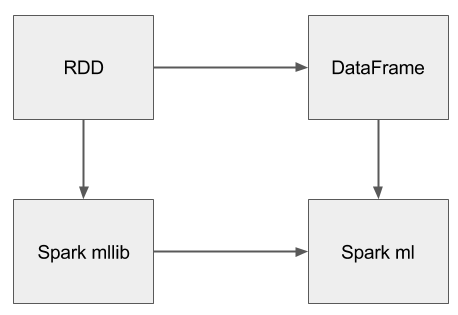
\includegraphics[height=4cm]{images/mllib-ml}
\end{center}

\end{frame}

\begin{frame}{Pipelines}
\begin{itemize}
\item Main concept of spark.ml.
\item Sequence of stages (estimators, transformers, models).
\item It is easy to maintain a Pipeline.
\item Used for feature engineering, cross-validation and model fitting.
\end{itemize}

\bigskip
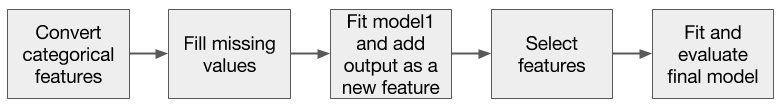
\includegraphics[width=12cm]{./images/pipeline}
\end{frame}


\begin{frame}{Estimators and transformers}
\begin{itemize}
\item Estimators use existing data to estimate parameters, for example categorical features. Learning algorithms are also estimators. Output of estimator is a transformer.
\item Adds new colums to a dataframe, such as new (engineered) feature or model output (estimation, probability, etc.). 
\end{itemize}
\end{frame}

\begin{frame}[fragile]{Estimators and transformers: example}

{\footnotesize
\begin{minted}{scala}
// Define indexers and encoders
val fieldsToIndex = Array("gender", "language")
val indexers = fieldsToIndex.map(f => new StringIndexer()
  .setInputCol(f).setOutputCol(f + "_index"))

val fieldsToEncode = Array("gender", "language")
val oneHotEncoders = fieldsToEncode.map(f => new OneHotEncoder()
  .setInputCol(f + "_index").setOutputCol(f + "_flags"))

val featureAssembler = new VectorAssembler()
  .setInputCols(Array("gender_flags", "language_flags"))
  .setOutputCol("features")

// Combine stages into pipeline
val pipeline = new Pipeline()
  .setStages(indexers ++ oneHotEncoders :+ featureAssembler)
\end{minted}
}
\end{frame}

\begin{frame}[fragile]{Estimators and transformers: example}

{\footnotesize
\begin{minted}{scala}
val data = sc.parallelize(Array(
  ("M", "EN", 1.0),
  ("M", "ES", 0.0),
  ("F", "EN", 1.0),
  ("F", "ZH", 0.1)
)).toDF("gender", "language", "label")

pipeline.fit(data).transform(data)
  .drop("gender_flags").drop("language_flags")
  .show()
\end{minted}

\begin{minted}{bash}
+------+--------+-----+------------+--------------+-------------+
|gender|language|label|gender_index|language_index|     features|
+------+--------+-----+------------+--------------+-------------+
|     M|      EN|  1.0|         0.0|           0.0|[1.0,1.0,0.0]|
|     M|      ES|  0.0|         0.0|           1.0|[1.0,0.0,1.0]|
|     F|      EN|  1.0|         1.0|           0.0|[0.0,1.0,0.0]|
|     F|      ZH|  0.1|         1.0|           2.0|    (3,[],[])|
+------+--------+-----+------------+--------------+-------------+
\end{minted}
}
\end{frame}


\begin{frame}{Feature engineering}
\begin{columns}
\column{.25\textwidth}
\begin{center}
	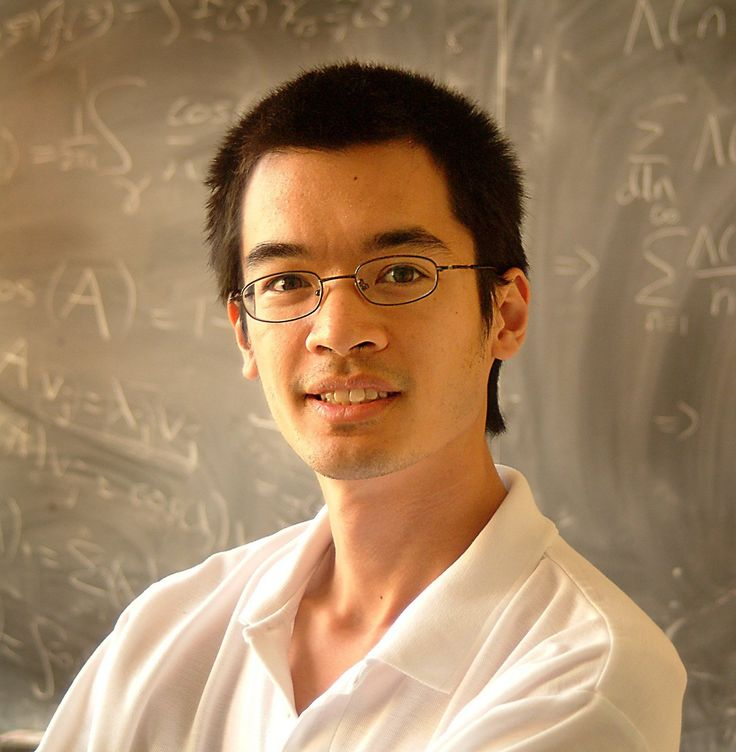
\includegraphics[width=3.2cm]{images/scientist}
\end{center}
\column{.75\textwidth}

\begin{itemize}
\item Feature creation is up to analyst. Spark is convenient from software engineering point of view, but not as practical as Python/R with in-memory dataframes.
\item Once features are defined, spark creates sparse vectors based on them. At this point only spark algorithms could be used. 
\end{itemize}
\end{columns}
\end{frame}

\begin{frame}[fragile]{Cross-validation and grid search example}

%{\scriptsize
{\footnotesize
\begin{minted}{scala}
val Array(training, test) = data.randomSplit(Array(0.9, 0.1), seed = 1234)

val featureAssembler = new VectorAssembler()
  .setInputCols(
    Array("sepal_length", "sepal_width", "petal_length", "petal_width")
  ).setOutputCol("features")
val lr = new LogisticRegression().setMaxIter(10)
val fullPipeline = new Pipeline().setStages(Array(featureAssembler, lr))

val paramGrid = new ParamGridBuilder()
  .addGrid(lr.regParam, Array(0.1, 0.01))
  .build()

val cv = new CrossValidator()
  .setEstimator(fullPipeline)
  .setEvaluator(new BinaryClassificationEvaluator)
  .setEstimatorParamMaps(paramGrid)
  .setNumFolds(5)

val cvModel = cv.fit(training)
\end{minted}
}
\end{frame}

\begin{frame}[fragile]{Cross-validation and grid search example}

%{\scriptsize
{\footnotesize
\begin{minted}{scala}
cvModel.transform(test)
    .select("features", "label", "prediction", "probability")
    .show()
\end{minted}

\begin{minted}{bash}
+-----------------+-----+----------+--------------------+
|         features|label|prediction|         probability|
+-----------------+-----+----------+--------------------+
|[5.9,3.0,4.2,1.5]|  0.0|       0.0|[0.80461154054846...|
|[5.5,2.4,3.8,1.1]|  0.0|       0.0|[0.92788428007362...|
|[5.8,2.7,3.9,1.2]|  0.0|       0.0|[0.91612929982336...|
|[6.0,2.7,5.1,1.6]|  0.0|       1.0|[0.42013327746284...|
|[6.0,2.9,4.5,1.5]|  0.0|       0.0|[0.71645104521227...|
|[6.7,3.0,5.0,1.7]|  0.0|       1.0|[0.46088659238049...|
|[6.4,2.7,5.3,1.9]|  1.0|       1.0|[0.21021735245935...|
|[7.6,3.0,6.6,2.1]|  1.0|       1.0|[0.03313839499693...|
|[6.4,3.2,5.3,2.3]|  1.0|       1.0|[0.11969201314865...|
|[6.0,3.0,4.8,1.8]|  1.0|       1.0|[0.45195167667592...|
|[7.7,3.0,6.1,2.3]|  1.0|       1.0|[0.04122882687014...|
+-----------------+-----+----------+--------------------+
\end{minted}
}
\end{frame}

\begin{frame}{Available algorithms}
\begin{columns}
\column{.25\textwidth}
\begin{center}
	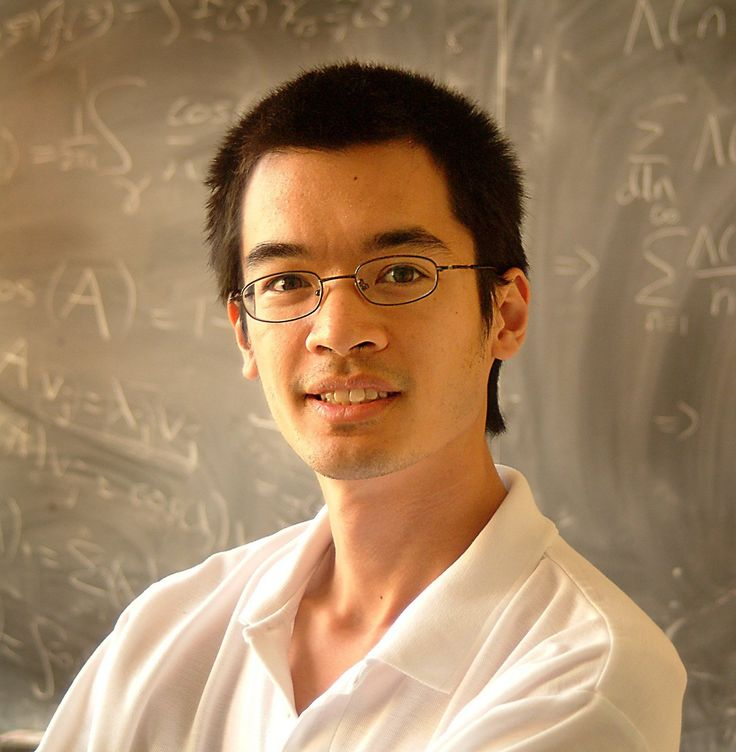
\includegraphics[width=3.2cm]{images/scientist}
\end{center}
\column{.75\textwidth}

\begin{itemize}
\item Spark is processing engine on top of \textbf{distributed} system. Not every algorithm is scalable, so spark.ml does not have them.
\item Current spark.ml algorithms: logistic regression, decision tree, neural network.
\item Interface is convenient, but speed and quality are not as good as xgboost.
\end{itemize}
\end{columns}
\end{frame}


\begin{frame}{Workflow}
\begin{center}
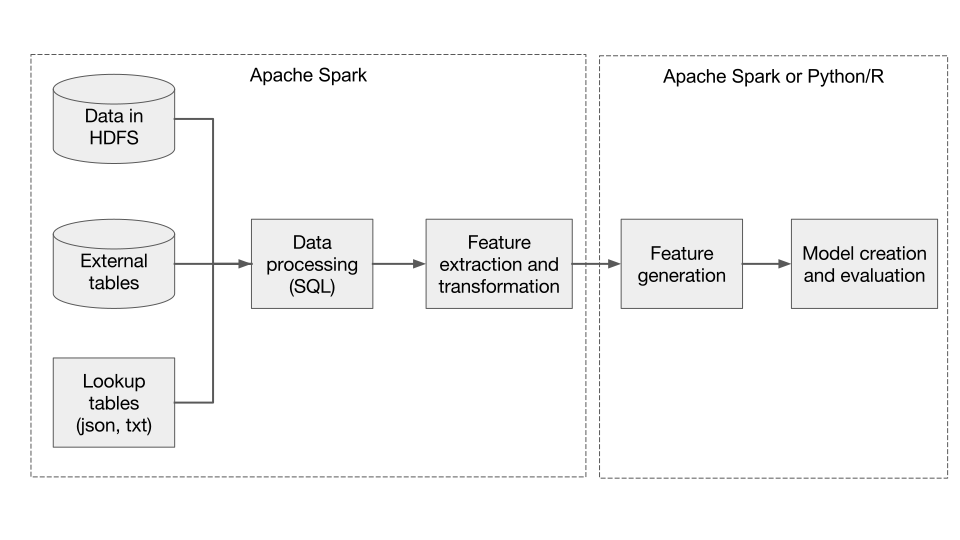
\includegraphics[width=12cm]{images/ml-workflow}
\end{center}
\end{frame}


\section{Conclusion}
\begin{frame}{Table of content}
\tableofcontents[currentsection]
\end{frame}

\begin{frame}{Conclusion}
\begin{itemize}
\item Spark is a good tool, but not for every task.
\item Data manipulation is easy and fast with Spark.
\item It's machine learning library is well designed, but accuracy is not as good as for in-memory solutions (xgboost/deep learning).
\end{itemize}
\end{frame}

\begin{frame}{Quiz}
\begin{enumerate}
\item<1-> Does spark have visualization module? \\
	\only<1>{A) Yes B) No}
	\only<2->{A) Yes B) \alert{No}}
\item<3-> Main concept of spark.ml is: \\
	\only<3>{A) Pipeline  B) Estimator C) Transformer D) Model}
	\only<4->{A) \alert{Pipeline}  B) Estimator C) Transformer D) Model}
\end{enumerate}
\end{frame}

\begin{frame}
\begin{center}
{\huge Thank you!}

\vfill
Kirill Pavlov, Data Science Team, Asia Miles Limited

kirill\_pavlov@asiamiles.com

{\small
%source code \href{https://gist.github.com/pavlov99/25a5cab2ab0199a27300b070cb1e02c7}{gist}
}
\end{center}
\end{frame}

\end{document}
